%%%%%%%%%%%%%%%%%%%%%%%%%%%%%%%%%%%%%%%%%
% Beamer Presentation
% LaTeX Template
% Version 2.0 (March 8, 2022)
%
% This template originates from:
% https://www.LaTeXTemplates.com
%
% Author:
% Vel (vel@latextemplates.com)
%
% License:
% CC BY-NC-SA 4.0 (https://creativecommons.org/licenses/by-nc-sa/4.0/)
%
%%%%%%%%%%%%%%%%%%%%%%%%%%%%%%%%%%%%%%%%%

%----------------------------------------------------------------------------------------
%	PACKAGES AND OTHER DOCUMENT CONFIGURATIONS
%----------------------------------------------------------------------------------------

\documentclass[
	11pt, % Set the default font size, options include: 8pt, 9pt, 10pt, 11pt, 12pt, 14pt, 17pt, 20pt
	%t, % Uncomment to vertically align all slide content to the top of the slide, rather than the default centered
	%aspectratio=169, % Uncomment to set the aspect ratio to a 16:9 ratio which matches the aspect ratio of 1080p and 4K screens and projectors
]{beamer}

\graphicspath{{Images/}{./}} % Specifies where to look for included images (trailing slash required)

\usepackage{tikz}
\usepackage{booktabs} % Allows the use of \toprule, \midrule and \bottomrule for better rules in tables
\urlstyle{same}

%----------------------------------------------------------------------------------------
%	SELECT LAYOUT THEME
%----------------------------------------------------------------------------------------

% Beamer comes with a number of default layout themes which change the colors and layouts of slides. Below is a list of all themes available, uncomment each in turn to see what they look like.

%\usetheme{default}
%\usetheme{AnnArbor}
%\usetheme{Antibes}
%\usetheme{Bergen}
%\usetheme{Berkeley}
%\usetheme{Berlin}
%\usetheme{Boadilla}
%\usetheme{CambridgeUS}
%\usetheme{Copenhagen}
%\usetheme{Darmstadt}
%\usetheme{Dresden}
%\usetheme{Frankfurt}
%\usetheme{Goettingen}
%\usetheme{Hannover}
%\usetheme{Ilmenau}
%\usetheme{JuanLesPins}
%\usetheme{Luebeck}
\usetheme{Madrid}
%\usetheme{Malmoe}
%\usetheme{Marburg}
%\usetheme{Montpellier}
%\usetheme{PaloAlto}
%\usetheme{Pittsburgh}
%\usetheme{Rochester}
%\usetheme{Singapore}
%\usetheme{Szeged}
%\usetheme{Warsaw}

%----------------------------------------------------------------------------------------
%	SELECT COLOR THEME
%----------------------------------------------------------------------------------------

% Beamer comes with a number of color themes that can be applied to any layout theme to change its colors. Uncomment each of these in turn to see how they change the colors of your selected layout theme.

%\usecolortheme{albatross}
%\usecolortheme{beaver}
%\usecolortheme{beetle}
%\usecolortheme{crane}
%\usecolortheme{dolphin}
%\usecolortheme{dove}
%\usecolortheme{fly}
%\usecolortheme{lily}
%\usecolortheme{monarca}
%\usecolortheme{seagull}
%\usecolortheme{seahorse}
%\usecolortheme{spruce}
%\usecolortheme{whale}
%\usecolortheme{wolverine}

\definecolor{mathpink}{RGB}{239, 96, 173}
\usecolortheme[named=mathpink]{structure}

%----------------------------------------------------------------------------------------
%	SELECT FONT THEME & FONTS
%----------------------------------------------------------------------------------------

% Beamer comes with several font themes to easily change the fonts used in various parts of the presentation. Review the comments beside each one to decide if you would like to use it. Note that additional options can be specified for several of these font themes, consult the beamer documentation for more information.

\usefonttheme{default} % Typeset using the default sans serif font
%\usefonttheme{serif} % Typeset using the default serif font (make sure a sans font isn't being set as the default font if you use this option!)
%\usefonttheme{structurebold} % Typeset important structure text (titles, headlines, footlines, sidebar, etc) in bold
%\usefonttheme{structureitalicserif} % Typeset important structure text (titles, headlines, footlines, sidebar, etc) in italic serif
%\usefonttheme{structuresmallcapsserif} % Typeset important structure text (titles, headlines, footlines, sidebar, etc) in small caps serif

%------------------------------------------------

%\usepackage{mathptmx} % Use the Times font for serif text
\usepackage{palatino} % Use the Palatino font for serif text

%\usepackage{helvet} % Use the Helvetica font for sans serif text
\usepackage[default]{opensans} % Use the Open Sans font for sans serif text
%\usepackage[default]{FiraSans} % Use the Fira Sans font for sans serif text
%\usepackage[default]{lato} % Use the Lato font for sans serif text

%----------------------------------------------------------------------------------------
%	SELECT INNER THEME
%----------------------------------------------------------------------------------------

% Inner themes change the styling of internal slide elements, for example: bullet points, blocks, bibliography entries, title pages, theorems, etc. Uncomment each theme in turn to see what changes it makes to your presentation.

%\useinnertheme{default}
\useinnertheme{circles}
%\useinnertheme{rectangles}
%\useinnertheme{rounded}
%\useinnertheme{inmargin}

%----------------------------------------------------------------------------------------
%	SELECT OUTER THEME
%----------------------------------------------------------------------------------------

% Outer themes change the overall layout of slides, such as: header and footer lines, sidebars and slide titles. Uncomment each theme in turn to see what changes it makes to your presentation.

%\useoutertheme{default}
%\useoutertheme{infolines}
%\useoutertheme{miniframes}
%\useoutertheme{smoothbars}
%\useoutertheme{sidebar}
%\useoutertheme{split}
%\useoutertheme{shadow}
%\useoutertheme{tree}
%\useoutertheme{smoothtree}

%\setbeamertemplate{footline} % Uncomment this line to remove the footer line in all slides
%\setbeamertemplate{footline}[page number] % Uncomment this line to replace the footer line in all slides with a simple slide count

%\setbeamertemplate{navigation symbols}{} % Uncomment this line to remove the navigation symbols from the bottom of all slides

%----------------------------------------------------------------------------------------
%	PRESENTATION INFORMATION
%----------------------------------------------------------------------------------------

\title[Ramsey Theory with Ultrafilters]{Ramsey Theory with Ultrafilters} % The short title in the optional parameter appears at the bottom of every slide, the full title in the main parameter is only on the title page

\subtitle{} % Presentation subtitle, remove this command if a subtitle isn't required

\author[Megan W. \and Yanna J.]{Megan Winterburn, Yanna Jaskielewicz \\ Mentor: Jashan Bal} % Presenter name(s), the optional parameter can contain a shortened version to appear on the bottom of every slide, while the main parameter will appear on the title slide

\institute[UW]{University of Waterloo} % Your institution, the optional parameter can be used for the institution shorthand and will appear on the bottom of every slide after author names, while the required parameter is used on the title slide and can include your email address or additional information on separate lines

\date[\today]{WiM Directed Reading Program \\ \today} % Presentation date or conference/meeting name, the optional parameter can contain a shortened version to appear on the bottom of every slide, while the required parameter value is output to the title slide

%----------------------------------------------------------------------------------------

\begin{document}

%----------------------------------------------------------------------------------------
%	TITLE SLIDE
%----------------------------------------------------------------------------------------

\begin{frame}
	\titlepage % Output the title slide, automatically created using the text entered in the PRESENTATION INFORMATION block above
\end{frame}

%----------------------------------------------------------------------------------------
%	TABLE OF CONTENTS SLIDE
%----------------------------------------------------------------------------------------

% The table of contents outputs the sections and subsections that appear in your presentation, specified with the standard \section and \subsection commands. You may either display all sections and subsections on one slide with \tableofcontents, or display each section at a time on subsequent slides with \tableofcontents[pausesections]. The latter is useful if you want to step through each section and mention what you will discuss.

\begin{frame}
	\frametitle{Overview} % Slide title, remove this command for no title
	
	\tableofcontents % Output the table of contents (all sections on one slide)
	%\tableofcontents[pausesections] % Output the table of contents (break sections up across separate slides)
\end{frame}

%----------------------------------------------------------------------------------------
%	PRESENTATION BODY SLIDES
%----------------------------------------------------------------------------------------

% Introduction
\section{Introduction}

\begin{frame}
    \frametitle{Introduction to Ramsey Theory}

    What is Ramsey Theory?

    \vspace{10pt}

    \begin{quote}
		A branch of \dots combinatorics that focuses on the appearance of order in a substructure given a structure of a known size.\\
		--- Wikipedia
	\end{quote}

    \vspace{10pt}

    \begin{quote}
		Complete disorder is impossible.\\
		--- Theodore S. Motzkin
	\end{quote}

\end{frame}

\begin{frame}
    \frametitle{Introduction to Ramsey Theory}

    \begin{example}
        Suppose we have a group of six random people. Any two given people are either friends or strangers. Can we always find at least three people who are either all mutual friends or all strangers?

        \pause

        \begin{center}
            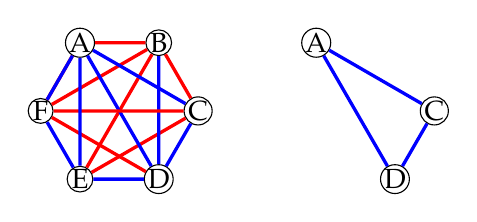
\begin{tikzpicture}[main/.style = {circle, draw=black, minimum size=1.5mm, inner sep=0pt, node distance=1.5cm}]
                \begin{scope}[shift={(-1.5cm, 0)}]
                    \node[main] (1) at ( 60:1cm) {B};
                    \node[main] (2) at (120:1cm) {A};
                    \node[main] (3) at (180:1cm) {F};
                    \node[main] (4) at (240:1cm) {E};
                    \node[main] (5) at (300:1cm) {D};
                    \node[main] (6) at (360:1cm) {C};

                    \draw[red, very thick] (1) -- (2) -- (3) -- (1) -- (4) -- (6);
                    \draw[blue, very thick] (1) -- (5) -- (2) -- (3) -- (4) -- (5) -- (6);
                    \draw[red, very thick] (1) -- (6) -- (3) -- (5);
                    \draw[blue, very thick] (6) -- (2) -- (4);
                \end{scope}
                \begin{scope}[shift={(1.5cm, 0)}]
                    \node[main] (2) at (120:1cm) {A};
                    \node[main] (5) at (300:1cm) {D};
                    \node[main] (6) at (360:1cm) {C};

                    \draw[blue, very thick] (2) -- (5) -- (6) -- (2);
                \end{scope}
            \end{tikzpicture}
        \end{center}
    \end{example}
    
    \pause

    In every case, the answer is yes!
\end{frame}

\begin{frame}
    \frametitle{Infinite Ramsey Theory}

    We can extend similar notions to the infinitary case:

    \vspace{10pt}

    If we colour the edges of an infinite complete graph either \textcolor{red}{red} or \textcolor{blue}{blue}, can we find an infinite complete \textit{monochromatic} subgraph?

    \pause

    \begin{center}
        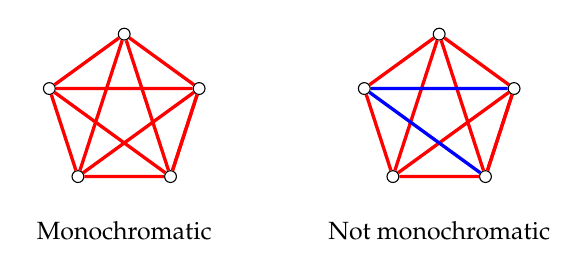
\begin{tikzpicture}[main/.style = {circle, draw=black, minimum size=1.5mm, inner sep=0pt, node distance=1.5cm}]
            \begin{scope}[shift={(-2cm, 0)}]
                \node[main] (1) at ( 90:1cm) {};
                \node[main] (2) at (162:1cm) {};
                \node[main] (3) at (234:1cm) {};
                \node[main] (4) at (306:1cm) {};
                \node[main] (5) at ( 18:1cm) {};

                \draw[red, very thick] (1) -- (2) -- (3) -- (4) -- (5) -- (1);
                \draw[red, very thick] (1) -- (3) -- (5) -- (4) -- (1);
                \draw [red, very thick] (4) -- (2) -- (5);

                \node at (0, -1.5) {\small{Monochromatic}};
            \end{scope}
                \begin{scope}[shift={(2cm, 0)}]
                \node[main] (1) at ( 90:1cm) {};
                \node[main] (2) at (162:1cm) {};
                \node[main] (3) at (234:1cm) {};
                \node[main] (4) at (306:1cm) {};
                \node[main] (5) at ( 18:1cm) {};

                \draw[red, very thick] (1) -- (2) -- (3) -- (4) -- (5) -- (1);
                \draw[red, very thick] (1) -- (3) -- (5) -- (4) -- (1);
                \draw [blue, very thick] (4) -- (2) -- (5);

                \node at (0, -1.5) {\small{Not monochromatic}};
            \end{scope}
        \end{tikzpicture}
    \end{center}

    \pause

    The answer is also yes - and we'll use ultrafilters as a tool to prove it!
\end{frame}

% Filters and ultrafilters
\section{Ultrafilters}

\begin{frame}
    \frametitle{Filters}
    An important tool for use in proving the Infinite Ramsey Theorem is a filter.
    \pause
    \begin{definition}
        A Filter \(\mathcal{F}\) on \(\mathbb{N}\) is a set of subsets of \(\mathbb{N}\) which satisfy the following conditions. 
        \pause
        \begin{enumerate}
            \item \(\mathcal{F}\) is non-empty and \(\emptyset \notin \mathcal{F}\)
            \item If A, B \(\in \mathcal{F} \) then \(A \cap B \in \mathcal{F}\)
            \item If \(A \in \mathcal{F}\) and \(B \in \mathcal{P}(\mathbb{N})\) satisfies \(A \subseteq B\) then \(B \in \mathcal{F}\)
        \end{enumerate}
    \end{definition}
\end{frame}

\begin{frame}
    \frametitle{Ultrafilters}
    Specifically, ultrafilters are useful. 
    \pause
    \begin{definition}
        An ultrafilter on \(\mathbb{N}\) is a maximal filter \(\mathcal{U} \subseteq \mathcal{P}(\mathbb{N})\) on \(\mathbb{N}\).
        i.e. if \(\mathcal{F}\) is another filter on \(\mathbb{N}\) such that \(\mathcal{U} \subseteq \mathcal{F}\) then \(\mathcal{U} = \mathcal{F}\).
    \end{definition}
\end{frame}

\begin{frame}
    \frametitle{Principal Ultrafilters}
    Some ultrafilters are principal,
    \pause
    \begin{definition}
        Fix \(n \in \mathbb{N}\).
        The filter \(\mathcal{F}_n\) is a principal ultrafilter if it contains all subsets of \(\mathbb{N}\) that include the element \(n\). 
    \end{definition}
    \pause
    though not all ultrafilters are principal, as we will show now. 
\end{frame}

\begin{frame}
    \frametitle{Existence of a Non-Principal Ultrafilter on \(\mathbb{N}\)}
    First consider the Fr\'echet Filter, defined as the set of all co-finite subsets.
    (i.e. it contains all power sets \(A\) of the natural numbers such that \(\mathbb{N} \setminus A\) is finite.)
    \pause
    \vspace{10pt}
    \break It can be proven with Zorn's Lemma that if \(\mathcal{F}\) is a filter on \(\mathbb{N}\), then there exists an ultrafilter \(\mathcal{U}\) such that \(\mathcal{F} \subseteq \mathcal{U}\)
    \pause
    \vspace{10pt}
    \break Applying this to the Fr\'echet Filter is used to prove the existence of a non-principal ultrafilter. 
    This is since there must be an ultrafilter, \(\mathcal{U}\) containing the Fr\'echet Filter. \break
    \pause
    Then if \(A \subseteq \mathbb{N}\) is a finite set it cannot be in \(\mathcal{U}\). \break
    Then by definition of the Fr\'echet Filter, \(\mathbb{N} \setminus A\) is in the Fr\'echet Filter which is a subset of \(\mathcal{U}\). \break
    So \(\mathcal{U}\) cannot be a principal ultrafilter. 
\end{frame}

\begin{frame}
    \frametitle{Important Property of Ultrafilters (1)}
    \begin{block}{}
		Let \(\mathcal{F}\) be a filter on \(\mathbb{N}\). Then \(\mathcal{F}\) is an ultrafilter if and only if for every \(A \subseteq \mathbb{N}\), either \(A \in \mathcal{F}\) or \(\mathbb{N} \setminus A \in \mathcal{F}\).
	\end{block}

\end{frame}

\begin{frame}
    \frametitle{Important Property of Ultrafilters (2)}
    \begin{block}{}
    Let \(\mathcal{U}\) be an ultrafilter on \(\mathbb{N}\) and \(A_1, A_2, ..., A_n \subseteq \mathbb{N}\).
    \pause
    \vspace{10pt}
    \break If \(A_1 \cup A_2 \cup ... \cup A_n = \bigcup\limits_{i=1}^{n} A_{i} \in \mathcal{U}\),
    \vspace{10pt}
    \break then there exists \(1 \leq j \leq n\), such that \(A_j \in \mathcal{U}\).
    \end{block}
    \pause
    \vspace{10pt}
    If \(\mathcal{U}\) is non-principal, then we get a useful result:\\
    \vspace{10pt}
    % Note: the square cup means its a disjoint union (hence a partition)
    If \(A_1 \sqcup \cdot \cdot \cdot \sqcup A_n = \mathbb{N}\) is a partition, then exactly one of \(A_j \in \mathcal{U}\).
\end{frame}

% Filters and ultrafilters
\section{Infinite Ramsey's Theorem}
\begin{frame}
    \frametitle{Proof of Infinite Ramsey Theorem}
    The proof is quite long so we will provide a general idea.
    \pause
    \vspace{10pt}
    \break Consider the complete graph on the natural numbers, a red-blue colouring on this graph, and \(\mathcal{U}\), a non-principal ultrafilter on \(\mathbb{N}\).
    \vspace{10pt}
    \pause
    Fixing a particular vertex \(v\) we can partion \(\mathbb{N}\) into a set containing:
    \pause
    \begin{enumerate}
        \item \(v\) itself 
        \item a set containing all vertices which share a red edge with \(v\)
        \item and a set containing all vertices which share a blue edge with \(v\)
    \end{enumerate}

    \vspace{10pt}

    \pause

     Now since \(\mathcal{U}\) is non-principal the set only containing \(v\) is not in \(\mathcal{U}\).
     So it must be that one of the other sets is by the second important property we provided above.
     If, for example, it is the blue set you can keep picking vertices infinitely in that set which are in their blue set to get a monochromatic subgraph.
     The same applies for if it is the red set. 
\end{frame}
% Idempotent ultrafilters
\section{Idempotent Ultrafilters and Finite Sums}

\begin{frame}
    \frametitle{Ultrafilter Addition}
    \begin{definition}
        Given \(A \subseteq \mathbb{N}\) and \(n \in \mathbb{N}\), define \(A-n\) as the shifted subset given by
        \[A-n = \{m \in \mathbb{N}: n + m \in A\}.\]
    \end{definition}

    \vspace{10pt}

    \pause 

    We can extend this notion to define addition between ultrafilters:\\[10pt]

	\begin{definition}
        Let \(\mathcal{U}\) and \(\mathcal{W}\) be ultrafilters on \(\mathbb{N}\). We define \(\mathcal{W} + \mathcal{U}\) such that for all \(A \subseteq \mathbb{N}\), we have that \(A \in \mathcal{W} + \mathcal{U}\) if and only if
        \[\{n \in \mathbb{N}: A - n \in \mathcal{W} \} \in \mathcal{U}.\]
    \end{definition}

    \vspace{10pt}

    Importantly, we get that \(\mathcal{W} + \mathcal{U}\) is also an ultrafilter.
\end{frame}

\begin{frame}
    \frametitle{Properties of Ultrafilter Addition}

    \begin{example}
        If \(\mathcal{U}_n\) and \(\mathcal{U}_m\) are the principal ultrafilters associated to \(n\in \mathbb{N}\) and \(m \in \mathbb{N}\), respectively, then \(\mathcal{U}_n + \mathcal{U}_m = \mathcal{U}_{n+m}\).
    \end{example}

    \pause

    \vspace{10pt}

    In this example, \(\mathcal{U}_n + \mathcal{U}_m = \mathcal{U}_{n+m} = \mathcal{U}_m + \mathcal{U}_n\). So, it might be natural to assume that ultrafilter addition is associative.

    \pause

    \vspace{10pt}

    \begin{block}{Non-Associativity}
        Ultrafilter addition is not associative. For any ultrafilters \(\mathcal{U}\) and \(\mathcal{W}\), it is not generally true that \(\mathcal{W} + \mathcal{U} = \mathcal{U} + \mathcal{W}\).
    \end{block}
\end{frame}

\begin{frame}
	\frametitle{Idempotent Ultrafilters} % Slide title, remove this command for no title

	\begin{lemma}[Ellis-Nakamura Lemma]
        There exists a non-principal ultrafilter \(\mathcal{U}\) on \(\mathbb{N}\) such that \(\mathcal{U} + \mathcal{U} = \mathcal{U}\). That is, \(\mathcal{U}\) is said to be idempotent.
    \end{lemma}

    \vspace{10pt}
    \pause
    Then if \(\mathcal{U}\) is idempotent with \(A \in \mathcal{U}\): \pause
    \begin{itemize}
        \item \(A \in \mathcal{U} + \mathcal{U}\)
        \item \(\{n \in \mathbb{N}: A - n \in \mathcal{U}\} \in \mathcal{U}\)
    \end{itemize}

    \pause
    \vspace{10pt}
    So, we can define \[A^* = A \cap \{n \in \mathbb{N}: A - n \in \mathcal{U}\},\] and we have that \(A^* \in \mathcal{U}\)!
\end{frame}

\begin{frame}
    \frametitle{Finite Sums}

    \begin{definition}
        Given a subset \(M \subseteq \mathbb{N}\), the finite sums of \(M\) is the subset FS\((M) \subseteq \mathbb{N}\) such that
        \[\text{FS}(M) = \Big\{ \sum_{x\in I} x : I \subseteq M \text{ finite nonempty subset} \Big\}.\]
    \end{definition}

    \pause

    \begin{example}
        Given \(x,y \in \mathbb{N}\), the finite sums of \(x\) and \(y\) are 
        \[\text{FS}(\{x, y\}) = \{x, y, x+y\}.\]
    \end{example}
\end{frame}

\begin{frame}
    \frametitle{Schur's Theorem}
    \begin{theorem}[Schur's Theorem]
        Given any 2-colouring \(\gamma: \mathbb{N} \to \{\text{\textcolor{red}{red}}, \text{\textcolor{blue}{blue}}\}\), there exist distinct \(x,y \in \mathbb{N}\) such that \(\{x, y, x+ y\}\) is a monochromatic subset.
    \end{theorem}

    \pause

    \vspace{10pt}

    \textit{Proof}. Let \(\mathcal{U}\) be an idempotent ultrafilter on \(\mathbb{N}\) and let \(\gamma: \mathbb{N} \to \{\text{\textcolor{red}{red}}, \text{\textcolor{blue}{blue}}\}\) be a 2-colouring on \(\mathbb{N}\).
    \vspace{10pt}

    \pause
    
    So, we can define the sets \(A = \{n \in \mathbb{N}: \gamma(n) = \text{\textcolor{red}{red}}\}\) and \(B = \{n \in \mathbb{N}: \gamma(n) = \text{\textcolor{blue}{blue}}\}\) and observe that \(\mathbb{N} = A \sqcup B\).\\
    
    \vspace{10pt}

    \pause
    
    Then, exactly one of \(A\) or \(B\) is in \(\mathcal{U}\). Without a loss of generality, suppose that \(A \in \mathcal{U}\).
\end{frame}

\begin{frame}
    \frametitle{Proof of Schur's Theorem}

    Since \(\mathcal{U}\) is idempotent, we have \(A^* = A \cap \{n \in \mathbb{N}: A - n \in \mathcal{U}\} \in \mathcal{U}\). So, pick \(x_1 \in A^*\). We get that: \pause

    \begin{itemize}
        \item \(x_1 \in A\)
        \item \(A-x_1 \in \mathcal{U}\)
    \end{itemize}

    \pause

    \vspace{10pt}

    Let \(A_1 = A \cap (A-x_1)\) and pick \(x_2 \in A_1^* = A_1 \cap \{n \in \mathbb{N}: A_1 - n \in \mathcal{U} \}\). Then, we have: \pause
    \begin{itemize}
        \item \(x_2 \in A_1\), so \(x_2 \in A\)
        \item \(x_2 \in A-x_1\) \pause
    \end{itemize}

    \vspace{10pt}

    Since \(x_2 \in A - x_1\), we have that \(x_1 + x_2 \in A\).\\
    
    \vspace{10pt}

    So \(x_1, x_2\), and \(x_1 + x_2\) are all \(\gamma\)-\textcolor{red}{red}!

\end{frame}

\begin{frame}
    \frametitle{Hindman's Theorem}

    We can carry on such a construction indefinitely to obtain an \textit{infinite} subset.

    \begin{theorem}[Hindman's Theorem]
        Let \(\gamma: \mathbb{N} \to \{\text{\textcolor{red}{red}}, \text{\textcolor{blue}{blue}}\}\) be a 2-colouring of \(\mathbb{N}\). Then there exists an infinite subset \(M \subseteq \mathbb{N}\) such that FS(\(M\)) is monochromatic.
    \end{theorem}

\end{frame}

\begin{frame}
    \frametitle{Further Applications}

    We focused on infinite sets in our examples, specifically \(\mathbb{N}\). But what about finite cases?

    \pause

    \vspace{10pt}

    Our infinite results can be used to prove their finite counterparts!
\end{frame}

\begin{frame} % Use [allowframebreaks] to allow automatic splitting across slides if the content is too long
	\frametitle{References}
	
	\begin{thebibliography}{99} % Beamer does not support BibTeX so references must be inserted manually as below, you may need to use multiple columns and/or reduce the font size further if you have many references
		\footnotesize % Reduce the font size in the bibliography
			
		\bibitem[DFB]{p1}
			David J. Fernandez-Bréton
			\newblock Using ultrafilters to prove Ramsey-type theorems
			\newblock \emph{American Mathematical Monthly} 129 no. 2 (2022), 116-131

		\bibitem[JB]{p2}
			Jashan Bal
			\newblock Ramsey theory
        
		\bibitem[TG]{p3}
            Timothy Gowers
			\newblock How to use ultrafilters
            \newblock \url{https://www.tricki.org/article/How_to_use_ultrafilters}

		\bibitem[VT]{p4}
            Veselin Jungic
			\newblock Introduction to Ramsey Theory

	\end{thebibliography}
\end{frame}

\end{document}